%%%%%%%%%%%%%%%%%%%%%%%%%%%%%%%%%%%%%%%%%%%%%%%%%%%%%%%%%%%%%%%%%%%%%%%%%%%

\documentclass[a4paper,oneside,12pt]{article}
\usepackage{mystyle}

\begin{document}

\title{\Large\bf Linear functions}
\author{%%
  Minh Van Nguyen \\
  \url{mvngu@gmx.com}
}
\date{\today}
\maketitle

\begin{packeditem}
\item General form of linear equations.

\item Constant function $y = a$.

\item Special function $y = x$.

\item Graph of linear function.

\item Application of linear equations: fill a bucket with water.
\end{packeditem}

%%%%%%%%%%%%%%%%%%%%%%%%%%%%%%%%%%%%%%%%%%%%%%%%%%%%%%%%%%%%%%%%%%%%%%%%%%%

\section{General form}

A \emph{linear function} is an expression of the form
%%
\begin{equation}
\label{eqn:linear_function_general}
f(x)
=
ax + b.
\end{equation}
%%
The numbers $a$ and $b$ are fixed real numbers, while $x$ is a
variable that can be any real number.  What does the function $f(x)$
look like?

As an example, set $a = b = 1$ so that you have $f(x) = x + 1$.  The
graph of $f(x) = x + 1$ is a straight line that passes through the
point $A = \tuple{-1}{0}$ on the $x$-axis and the point
$B = \tuple{0}{1}$ on the $y$-axis.  How were the coordinates of $A$
and $B$ calculated?  For the point $A$, you set $f(x) = 0$ and solve
the equation $0 = x + 1$ for $x$ to get $x = -1$.  The $x$-coordinate
of $A$ is $-1$ and the $y$-coordinate is $0$.  For the point $B$,
you set $x = 0$ and solve the equation $y = 0 + 1$ for $y$ to obtain
$y = 1$.  Then $B$ has $x$-coordinate $0$ and $y$-coordinate $1$.  You
plot the points $A$ and $B$, then draw a straight line through those
two points to produce the graph in \Figure{fig:plot_x_+_1}.

\begin{figure}[!htbp]
\centering
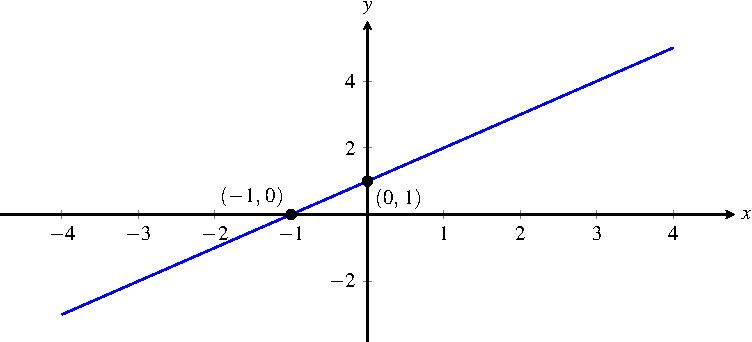
\includegraphics[scale=1]{image/06/a-1-b-1.pdf}
\caption{%%
  A graph of the function $f(x) = x + 1$.
}
\label{fig:plot_x_+_1}
\end{figure}

In general, how would you draw the graph of the
\Function{eqn:linear_function_general}?  As in the example above, you
set $f(x) = 0$ and determine the point $A = \tuple{\alpha}{0}$, where
$x = \alpha$ is obtained by solving $f(x) = 0$ for $x$.  You then set
$x = 0$ and determine the point $B = \tuple{0}{\beta}$, where
$\beta = f(0)$.  Plot the points $A$ and $B$, then draw a straight
line through those two points.  The result is a graph of the
\Function{eqn:linear_function_general}.  Let's put the above strategy
into practice.

\end{document}
